\documentclass[journal]{IEEEtran}
\usepackage[pdftex]{graphicx}
\usepackage{amsfonts}
\usepackage{amsmath}
\usepackage{caption}
\usepackage{cite}

\begin{document}

\title{CS7IS3: Assignment \#1}
\author{Conor McCauley, 17323203}

\maketitle

\section{Introduction}

The search engine program is written in \textit{Java 1.7} and utilises \textit{Apache Lucene 8.10.0}. The program has three primary modes of operation: indexing, searching and scoring. The indexing mode can parse the \textit{Cranfield Collection} corpus and add the included documents to a search index. The searching mode allows the user to interactively search the index for terms and phrases and will output the most relevant results. The scoring mode will grade the search engine using the list of queries provided with the \textit{Cranfield Collection} and output the results to a local file.

The user can, via command line arguments, specify the type of analyser to index the corpus with, the scoring method used to determine the most relevant search results and the type of parser to use when handling queries. The precise operation of the program and its command line arguments are described in the \textit{`readme'} file located on the virtual machine.

\section{Implementation}

\subsection{Driver Function}

The \textit{Cranfield} class contains the program's driver function: \textit{main()}. This function uses the \textit{Apache Commons CLI} library to parse command line arguments. The command line arguments are used to specify the operating mode, the analyser, the scoring method and the query parser.

The operating modes were described in the previous section. The standard analyser provided by \textit{Lucene} will be used by default but a custom-made analyser can be specified instead. Similarly, a \textit{BM25} scoring function will be used by default but a \textit{VSM} function can be used instead. Finally, the standard query parser will be used by default but a multi-field query parser can be used instead.

Provided the command line arguments are valid, the driver function will instantiate an instance of the \textit{Cranfield} class with the appropriate analyser and pass this instance to the relevant function for the given operating mode.

\subsection{Document Parsing}

The document parser reads each line from the corpus file into a list of strings. It then instantiates an empty list of \textit{Lucene} documents. Each document in the corpus contains an index header as well as numerous sub-headers for the document's title, author, abstract and what appears to be a department or publication.

The basic operation of the parser is to maintain a buffer with the current document and document field being parsed. A new document is denoted by the index header \texttt{.I} while the document fields are denoted by similar headers: \texttt{.T}, \texttt{.A}, \textit{etc.}. When a new field header is reached the previous field is added to the current document and the new field begins being parsed. When a new index header is reached the current field is added to the document and that document is added to the aforementioned list of documents and an empty one is instantiated in its place.

In a handful of cases, an individual document may contain what appears to be additional author, abstract or department headers within the original abstract section of the text. These elements of the text are simply included in the abstract field using some basic flagging logic.

\subsection{Indexing}

Indexing occurs once the corpus has been parsed into a list of \textit{Lucene} documents. The index directory is opened and an \textit{IndexWriter} is instantiated and used to write each of the parsed documents to the index. The index writer receives the analyser whose type was specified by the user as a configuration parameter.

The default analyser, as previously mentioned, is the \textit{StandardAnalyzer} which tokenises text by making it lowercase, removing a moderate amount of stop words and cutting up tokens of a certain maximum length. This analyser is also capable of recognising complex terms such as email addresses and URLs.

The custom analyser, which was designed for this program, tokenises text by making it lowercase, filtering out possessive tokens, removing a much larger amount of stop words\cite{ranksnl:stopwords} and normalising similar terms using a porter stemming filter.

The use of additional \textit{Lucene} analysers, such as the simple analyser, was considered. However, cursory testing showed that none of these options were nearly as suitable for this corpus as the default standard analyser so they were not implemented.

\subsection{Searching}

Searching is done from within the \textit{Searcher} class which can be used interactively by the user, via the \textit{interactive()} function, or called directly when grading the engine, via the \textit{search()} function.

The method for interactive searching simply consists of a loop that receives user queries from the command line and prints out the titles of the top five resulting documents as well as their scores. The method for direct searching takes a query string and an output buffer as parameters. It then runs the query and, using the output buffer, writes the results of the query to a results file in a format suitable for evaluation by \textit{TREC\_EVAL}.

\subsubsection{Scoring Function}

When the \textit{Searcher} class is instantiated an index searcher is created which uses either a \textit{Best Matching 25} scoring function, implemented as \textit{BM25Similarity}, or a \textit{Vector Space Model} scoring function, implemented as \textit{ClassicSimilarity}.

The VSM scoring function uses the classic TF-IDF statistic to rank documents based on how frequently query terms occur in a document in combination with how frequently these terms appear in all the documents. 

The BM25 scoring function is a probabilistic relevance model that combines elements of the TF-IDF statistic with the average length of documents in the corpus and individual weights for query terms.

\subsubsection{Query Parser}

Similarly, when the \textit{Searcher} class is instantiated a query parser is created using either the default \textit{QueryParser} or the more complex \textit{MultiFieldQueryParser}.

The default query parser is given a default search field, in our case the document abstract, and an analyser which it uses to extract terms from the query string. Although this parser supports advanced features such as wildcards and field-specific searches these features are unavailable to us given the simple nature of the provided query strings.

The multi-field query parser also uses an analyser to extract terms from the query string. However, this parser also allows us to `weight' the document fields when searching as opposed to simply having a default field. The parser boosts the importance of each field when determining the relevance of each document based on the provided scores/weights. The largest score was given to the abstract field with a smaller score given to the title field and an even smaller score given to the department field. The author field was not included as, based on a manual examination of the corpus and queries, it did not appear to have any relevance whatsoever on the search results.

\subsection{Scoring}

Scoring is done by parsing the queries file from the \textit{Cranfield Collection} into a list of strings using a much simpler version of the index document parser. An instance of the \textit{Searcher} class is then instantiated with the specified scoring function and query parser and an output buffer is created for the results file. The \textit{search()} method is then called for each query and the search results and scores are written to the results file as described in the previous section.

\section{Evaluation}

A shell script was used to run \textit{TREC\_EVAL} against the results from each combination of analyser, scoring function and query parser. The \textit{`mean average precision' (MAP)} and \textit{`set recall'} values were evaluated. The resulting values can be seen in figures 1 and 2, respectively.

The custom analyser outperforms the standard analyser in \textit{MAP} regardless of the scoring function and query parser. This is most likely due to the addition of more stop words and porter stemming in the custom analyser. In every case the engine using \textit{BM25} outperforms the \text{VSM} engine in \textit{MAP} which is to be expected given that it is considered to be a superior ranking system. In all but one case the multi-field parser outperforms the standard query parser. The optimal engine with regards to the \textit{MAP} seems to be the one using the custom analyser, \textit{BM25} and the multi-field parser with a value of $0.4401$.

Engines using the standard analyser have a moderately higher \textit{set recall} value than those using the custom analyser despite having worse \textit{MAP} values. This disparity is likely due to the standard analyser simply returning more results than the custom analyser leading to a lower precision (relevant retrieved results / total retrieved results) but a higher recall (relevant retrieved results / total relevant results).

\begin{figure}[!t]
\centering
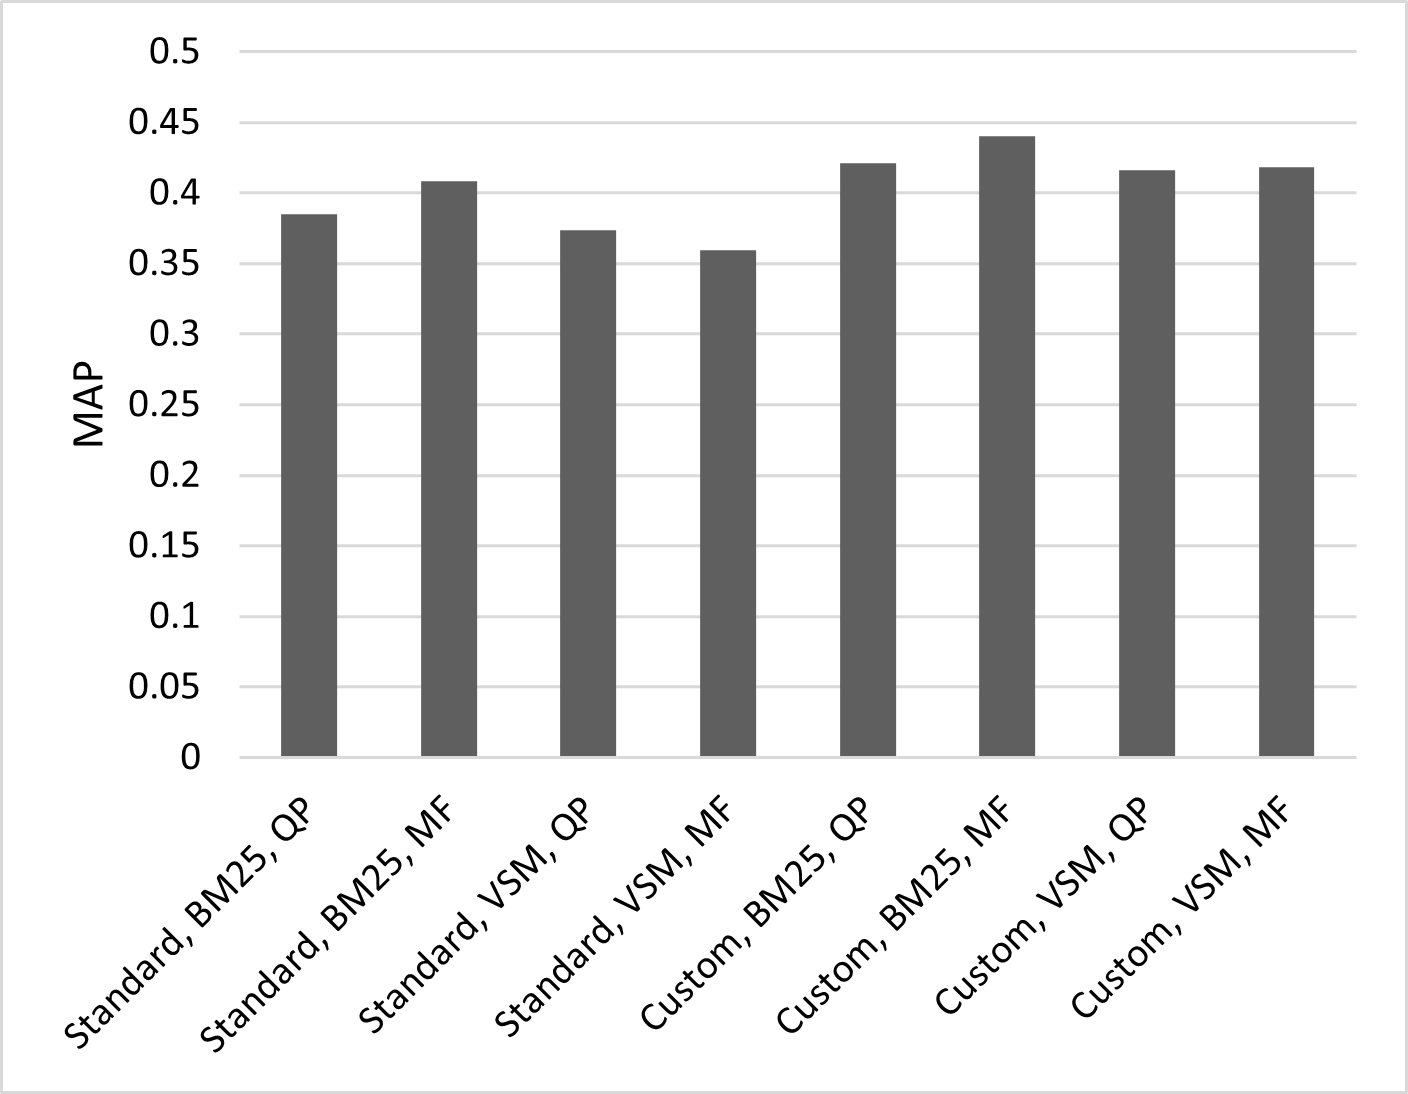
\includegraphics[width=3.2in]{graph_map.png}
\captionsetup{justification=centering}
\caption{MAP values for each engine}
\label{fig_sim}
\end{figure}

\begin{figure}[!t]
\centering
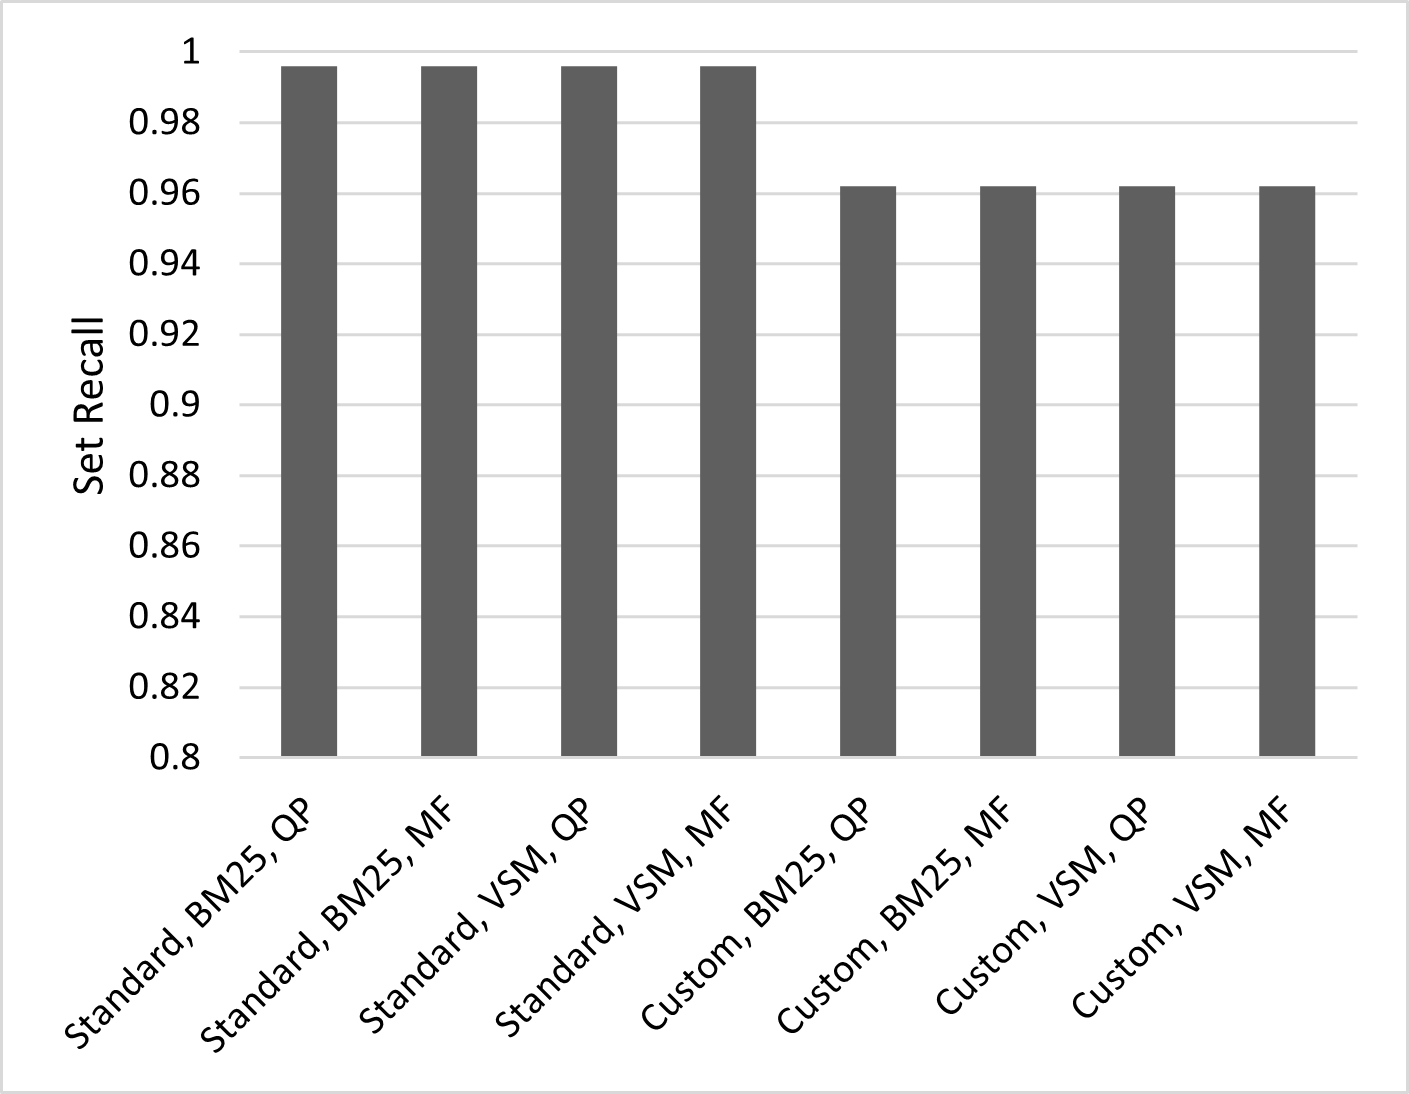
\includegraphics[width=3.2in]{graph_sr.png}
\captionsetup{justification=centering}
\caption{Set recall values for each engine}
\label{fig_sim}
\end{figure}

\begin{thebibliography}{1}

\bibitem{ranksnl:stopwords} Ranks NL, \emph{Default English stopwords list}, viewed 22 October 2021, $<$https://www.ranks.nl/stopwords$>$

\end{thebibliography}

\end{document}
